\documentclass[
  bibliography=totoc,     % Literatur im Inhaltsverzeichnis
  captions=tableheading,  % Tabellenüberschriften
  titlepage=firstiscover, % Titelseite ist Deckblatt
]{scrartcl}

% Paket float verbessern
\usepackage{scrhack}

% Warnung, falls nochmal kompiliert werden muss
\usepackage[aux]{rerunfilecheck}

% unverzichtbare Mathe-Befehle
\usepackage{amsmath}
% viele Mathe-Symbole
\usepackage{amssymb}
% Erweiterungen für amsmath
\usepackage{mathtools}

% Fonteinstellungen
\usepackage{fontspec}
% Latin Modern Fonts werden automatisch geladen
% Alternativ zum Beispiel:
%\setromanfont{Libertinus Serif}
%\setsansfont{Libertinus Sans}
%\setmonofont{Libertinus Mono}

% Wenn man andere Schriftarten gesetzt hat,
% sollte man das Seiten-Layout neu berechnen lassen
\recalctypearea{}

% deutsche Spracheinstellungen
\usepackage[english]{babel}


\usepackage[
  math-style=ISO,    % ┐
  bold-style=ISO,    % │
  sans-style=italic, % │ ISO-Standard folgen
  nabla=upright,     % │
  partial=upright,   % ┘
  warnings-off={           % ┐
    mathtools-colon,       % │ unnötige Warnungen ausschalten
    mathtools-overbracket, % │
  },                       % ┘
]{unicode-math}

% traditionelle Fonts für Mathematik
\setmathfont{Latin Modern Math}
% Alternativ zum Beispiel:
%\setmathfont{Libertinus Math}

\setmathfont{XITS Math}[range={scr, bfscr}]
\setmathfont{XITS Math}[range={cal, bfcal}, StylisticSet=1]

% Zahlen und Einheiten
\usepackage[
  locale=DE,                   % deutsche Einstellungen
  separate-uncertainty=true,   % immer Unsicherheit mit \pm
  per-mode=symbol-or-fraction, % / in inline math, fraction in display math
]{siunitx}

% chemische Formeln
\usepackage[
  version=4,
  math-greek=default, % ┐ mit unicode-math zusammenarbeiten
  text-greek=default, % ┘
]{mhchem}

% richtige Anführungszeichen
\usepackage[autostyle]{csquotes}

% schöne Brüche im Text
\usepackage{xfrac}

% Standardplatzierung für Floats einstellen
\usepackage{float}
\floatplacement{figure}{htbp}
\floatplacement{table}{htbp}

% Floats innerhalb einer Section halten
\usepackage[
  section, % Floats innerhalb der Section halten
  below,   % unterhalb der Section aber auf der selben Seite ist ok
]{placeins}

% Seite drehen für breite Tabellen: landscape Umgebung
\usepackage{pdflscape}

% Captions schöner machen.
\usepackage[
  labelfont=bf,        % Tabelle x: Abbildung y: ist jetzt fett
  font=small,          % Schrift etwas kleiner als Dokument
  width=0.9\textwidth, % maximale Breite einer Caption schmaler
]{caption}
% subfigure, subtable, subref
\usepackage{subcaption}

% Grafiken können eingebunden werden
\usepackage{graphicx}

% schöne Tabellen
\usepackage{booktabs}

% Verbesserungen am Schriftbild
\usepackage{microtype}

% Literaturverzeichnis
\usepackage[
  backend=biber,
  sorting=none,
]{biblatex}
% Quellendatenbank
\addbibresource{lit.bib}
\addbibresource{programme.bib}

% Hyperlinks im Dokument
\usepackage[
  german,
  unicode,        % Unicode in PDF-Attributen erlauben
  pdfusetitle,    % Titel, Autoren und Datum als PDF-Attribute
  pdfcreator={},  % ┐ PDF-Attribute säubern
  pdfproducer={}, % ┘
]{hyperref}
% erweiterte Bookmarks im PDF
\usepackage{bookmark}

% Trennung von Wörtern mit Strichen
\usepackage[shortcuts]{extdash}

% Listings zum Einbinden von Quellcode
\usepackage{listings}

% BraKet-Notation
\usepackage{braket}

% Feynman Slashed
\usepackage{slashed}

% New Commands Axel
% aquation = aligned equations
\newenvironment{aquation}{\begin{equation}\begin{aligned}}{\end{aligned}\end{equation}}
% \text{ .}/, 
\newcommand{\tp}{\text{ . }}
\newcommand{\tc}{\text{ , }}
% shorthand for 1/2 
\newcommand{\oh}{\frac{1}{2}}
\newcommand{\ih}{\frac{i}{2}}
% shorthand for f(x)=1/x 
\newcommand{\odiv}[1]{\frac{1}{#1}}
\newcommand{\idiv}[1]{\frac{i}{#1}}

%%%%% shorthands for left/right brackets (r for round, s for square, c for curly)
% round brackets
\newcommand{\lbr}{\left(}
\newcommand{\rbr}{\right)}
\newcommand{\brr}[1]{\left( #1 \right)}
% square brackets 
\newcommand{\lbs}{\left[}
\newcommand{\rbs}{\right]}
\newcommand{\brs}[1]{\left[ #1 \right]}
% curly brackets 
\newcommand{\lbc}{\left{}
\newcommand{\rbc}{\right}}
\newcommand{\brc}[1]{\left{ #1 \right}}
% put stuff like \\ , \\& , etc. into brackets (by putting it outside)
\newcommand{\brbr}[1]{\right. #1 \left.}

%%%%% mathcal L, O (for Lagrangian densities and and SMEFT operators)
\newcommand{\Lm}{\mathcal{L}}
\newcommand{\Om}{\mathcal{O}}

%%%%% horizintal .5mm
\newcommand{\hsf}{\hspace{0.5mm}}

\author{%
  Joel Koch\\%
  \href{mailto:joel.koch@tu-dortmund.de}{joel.koch@tu-dortmund.de}
  \and%
  % Felix Symma\\%
  % \href{mailto:felix.symma@tu-dortmund.de}{felix.symma@tu-dortmund.de}%
  Axel Vogt \\%
  \href{mailto:axel.vogt@udo.edu}{axel.vogt@udo.edu}
}
\publishers{University Dortmund - Facilty of Physics}


\subject{v64}
\title{Interferometry}
\date{%
  Execution: 16.12.2024
  \hspace{3em}
  Submission: DATUM
}

\begin{document}

\maketitle
\thispagestyle{empty}
\tableofcontents
\newpage

\section{Theorie}
\label{sec:Theorie}
Die folgende Theorie ist auf \cite{Anleitung44} basiert.

\subsection{Die Röntgenröhre}
\label{subsec:Röntgenröhre}
In diesem Versuch wird eine Röntgenröhre mit Cu-Anode verwendet. In dieser werden Elektronen aus einer Glühkathode in Richtung Cu-Anode beschleunigt. Die in die Cu-Anode einschlagenden Elektronen interagieren dann mit dem Kupfer, und zwar auf zweierlei Arten: Durch Stöße mit den Elektronen in den Kupferatomen werden diese auf höhere Niveaus angeregt. meistens werden die Atome sogar ionisiert. Dies macht Plätze auf niedrigeren Niveaus frei und führt damit dazu, dass Elektronen höherer Niveaus unter Emission von Röntgenstrahlung auf auf diese niedrigeren Niveaus zurückfallen. Außerdem wird bei der Bewegung der Elektronen im elektrischen Feld innerhalb des Kupfers Bremsstrahlung emittiert.\\
In diesem Versuch wird die $\text{K}_\alpha$-Linie von Kupfer verwendet, also jene Röntgenstrahlung, welche beim Niveauübergang von der zweiten auf die erste Schale entsteht. Sie besitzt eine Wellenlänge von $\lambda=1.54\text{Å}$. Um diese aus dem restlichen Spektrum der Röntgenröhre herauszufiltern, wird ein \textit{Göbelspiegel} verwendet. Dieser bündelt die Strahlung und filtert alle anderen Linien aus der Strahlung heraus.\\
Die Strahlung fällt nach dem Göbelspiegel auf eine Blende, dann auf die Probe und dann auf eine weitere Blende. Die Blenden dienen dazu, den eingestellten Glanzwinkel der einfallenden und den gemessenen Glanzwinkel der ausfallenden Strahlung zu variieren.\\
\\
Bei sehr geringen Winkeln (kleiner als $\alpha_g$) schießt die Strahlung über die Probe hinaus. Dies äußert sich in einem reskalierenden Faktor vor der gemessenen reflektierten Intensität, dem \textit{Geometriefaktor} 
\begin{aquation}
    G &\coloneqq \left\{ \begin{matrix}
        \frac{D \sin{\alpha_i}}{d_0} & \alpha_i < \alpha_g \\
        1 & \text{sonst}
    \end{matrix} \right. \tc
    \label{eq:Geometriefaktor}
\end{aquation}
mit der Probenlänge $D$ und der Strahlbreite $d_0$.

\subsection{Der komplexe Brechungsindex}
Dringt elektromagnetische Strahlung in ein nicht absorbierendes Material ein, so nimmt der Brechungsindex einen reellen Wert an. Die Dispersionsrelation nimmt dann die Form 
\begin{aquation}
    k(\omega) &= \odiv{c}\omega n(\omega)
\end{aquation}
Diese Relation taucht direkt in der ebenen Wellengleichung auf, welche die Form 
\begin{aquation}
    \psi(x,t) &= \psi_0 e^{i( k(\omega) x - \omega t)}
\end{aquation}
annimmt.\\
Anhand dieser Tatsache lässt sich durch einige grundlegende mathematische Überlegungen ableiten, wie die Dispersionsrelation für den Fall eines absorbierenden Materials auszusehen hat. Absorption führt in der Welleenfunktion nämlich bekanntermaßen zu einem komplexen Anteil in der ansonsten reellen Wellenzahl. Dieser Anteil führt in der Wellenfunktion zu einem zusätzlichen Faktor, welcher einer Exponentialfunktion mit reellem negativen Koeffizienten führt, welche wiederum dafür sorgt, dass die Amplitude der Wellenfunktion immer weiter gegen null abflacht.\\
Da die Wellenzahl linear im Brechungsindex ist, liegt es nahe, diesen komplexen Anteil mit in den Brechungsindex aufzunehmen. Der resultierende komplexe Brechungsindex nimmt dann die Form 
\begin{aquation}
    n(\omega) &= \chi+ i \kappa
\end{aquation}
an. Der Absorptionskoeffizient $\kappa$ ist ein Maß für die Abflachung der Wellenfunktion, während $\chi$ der Realteil des Brechungsindex ist.\\
Im Falle von Röntgenstrahlung ist der Realteil des Brechungsindex typischerweise $\chi = 1-\delta$, wobei $\delta$ typischerweise in der Größenordnung $10^{-6}$ liegt. Für diesen Fall, in dem der Realteil kleiner als $1$ ist, existiert ein kritischer Winkeln $\alpha_C$. Für Glanzwinkel $\alpha<\alpha_C$ tritt Totalreflexion auf. Aus dem Brechungsgesetz von Snellius 
\begin{aquation}
\label{eq:brechungsgesetz}
    n_1 \sin(\theta_1) &= n_2 \sin(\theta_2)
\end{aquation}
lässt sich der kritische Winkel als jener Einfallswinkel ableiten, bei welchem der transmittierte Strahl parallel zur Oberfläche verläuft, was dem Setzen von $\theta_2=\frac{\pi}{2}$ entspricht. Der Index $1$ ist dabei f[r Winkel und Brechungsindex vor der Streuung reserviert, während für den Fall danach der Index $2$ verwendet wird.\\
Da im vorliegenden Fall der kritische Winkel für kleine $\delta$ benötigt wird, lässt sich dieser zu 
\begin{aquation}
    \alpha_C &\approx \sqrt{2 \delta} \tp
    \label{eq:alpha_C}
\end{aquation}
Nach der Streuung am Versuchsobjekt zerteilt sich die Welle in eine transmittierte Welle (Label $t$) und eine reflektierte Welle (Label $r$), wodurch sich die Gesamtwelle zu 
\begin{aquation}
    \psi(x,t) &= t \psi_t (x,t) + r \psi_r (x,t) \tp
\end{aquation}
Der Transmissions- und der Reflexionskoeffizient ergeben sich nach den Fresnel-Gleichungen, welche sich aus dem Brechungsgesetz \autoref{eq:brechungsgesetz} ableiten lassen, zu 
\begin{aquation}
    t &= \frac{2 n_1 \sin(\alpha_i)}{n_1\sin(\alpha_i) + n_2\sin(\alpha_t)} \\
    r &= \frac{n_1 \sin(\alpha_i) - n_1 \sin(\alpha_t)}{n_1 \sin(\alpha_i) + n_2 \sin(\alpha_t)}
\end{aquation}

Diese Größen sind jedoch keine direkten Observablen, sondern Wahrscheinlichkeitsamplituden. Die physikalischen Größen sind die \textit{Reflektivität} $R \coloneqq |r|^2$ und die \textit{Transmission} $T \coloneqq |t|^2$.\\
Außerdem sind sie linear abhängig voneinander, verknüft über die Relation $1 = R + T$. Aus diesem Grund genügt es, eine der beiden Größen zu messen. Für den Fall $\alpha_i > 3 \alpha_C$ ergibt sich die Reflektivität zu
\begin{aquation}
    R &= \left(\frac{\alpha_C}{2 \alpha_i}\right) \tp
    \label{eq:Fresnel}
\end{aquation}


\subsection{Effekte in Mehrschichtsystemen}
Unter der Annahme mehrschichtiger Systeme treten weitere Effekte auf. Ihre Ursache liegt darin begründet, dass bei jedem Schichtübergang ein Teil der Welle reflektiert und ein Teil transmittiert wird. Der Gangunterschied zweier Teilwellen resultiert darin, dass diese miteinander interferieren.\\
Konstruktive Interferenz tritt generell immer dann auf, wenn die Welle nicht phasenverschoben ist. Bezüglich des Gangunterschieds bedeutet dies, dass wenn der Gangunterschied insgesamt ein Vielfachte von $\lambda$ ist, konstruktive Interferenz auftritt. Destruktive Interferenz hingegen tritt auf, wenn der Gangunterschied ein ungerades ganzzahliges Vielfaches von $\frac{\lambda}{2}$ ist.\\
In diesem Versuch gibt es nur zwei Schichten. 
Dieses Interferenzverhalten schlägt sich in der Reflektivität nieder. Diese ist proportional zu der in diesem Versuch gemessene Observable der reflektierten Intensität gemäß der Relation 
\begin{aquation}
    R &= \frac{I_\text{r}}{I_\text{tot}}
\end{aquation}
mit der totalen Intensität des emittierten Strahls $I_\text{tot}$. Nach den Gesetzen der Trigonometrie resultiert eine Änderung des Einfallswinkels in einer Änderung des Gangunterschieds. Wird also ein hinreichend großer Winkelbereich abgefahren, sollten mehrere Interferenzmini- und -maxima auftreten. Diese Schwingungen werden \textit{Kiessig-Oszillationen} genannt. Ein Beispielplot f[r diese ist in \autoref{fig:kiessig} zu sehen.
\begin{figure}
    \centering
    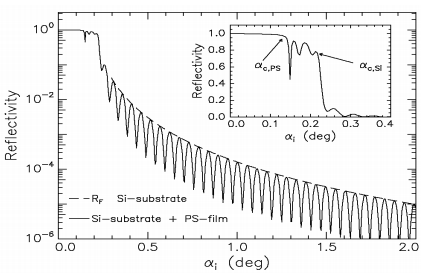
\includegraphics[width=\textwidth]{figures/kiessig.png}
    \caption{Kiessig-Oszillationen für einen Silizium-Wafer mit einer $800\si{\angstrom}$ dicken Polysterol-Schicht.}
    \label{fig:kiessig}
\end{figure} 

\subsection{Bestimmung der Schichtdicke}
Um die Dicke einer einzelnen Schicht zu bestimmen, wird die \textit{Bragg-Bedingung} 
\begin{aquation}
    n\lambda &= 2 d \sin(\alpha_i)
\end{aquation}
verwendet. Diese Gleichung setzt die Schicktdicke in Abhängigkeit des $n$-ten Minimums der Kiessig-Oszillation. Um diesen Parameter loszuwerden, wird die Differenz zwischen den Fällen $n+1$ und $n$ betrachtet. Da die hier verwendeten Glanzwinkel klein sind, kann der Sinus als $\sin(\alpha_i) \approx \alpha_i)$ genähert werden, sodass sich für die Differenz zweier benachbarter Interferenz-Extrema und damit direkt für die Schichtdicke die Formel 
\begin{aquation}
    d = \frac{\lambda}{2 \Delta\alpha_i}
\end{aquation}
ergibt.\\
Im Falle mehrerer Schichten überlagern sich aufgrund der Tatsache, dass es mehr als zwei Schichten gibt, mehrere austretenden Strahlen, welche unterschiedliche Anzahlen von Schichten durchlaufen haben, miteinander. Im Gegensatz dazu gab es bei einer einzelnen Schicht nur zwei Anteile: Den direkt reflektierten und den, welcher die eine Schicht durchlaufen hat.\\
Dies führt dazu, dass sich die Osziellationen aus allen Schichten ergeben, weswegen das Endergebnis nicht mehr direkt mit der Dicke einer einzelnen Schicht verbunden ist. Um die einzelnen Schichtdicken zu bekommen, gibt muss daher der \textit{Parrat-Algorithmus} verwendet werden. Dieser leitet sich her, indem das Amplitudenverhältnis $Q_j \coloneqq \frac{R_j}{T_j} = \frac{R_j}{1-R_j}$ zweier benachbarter Schichten an der $j$-ten Grenzfläche bestimmt wird. Da sich hier nämlich der Anteil der transmittierten Welle direkt von dem der reflektierten Welle ableiten lässt, lässt sich so durch Umstellen aus den Fresnel-Gleichungen direkt die Einfallende Welle für die folgende Grenzfläche bestimmen. Dies führt zu der Rekursionsformel 
\begin{aquation}
    Q_j &= e^{-2 i k_{z,j} z_j}\frac{r_{j,j+1} + Q_j e^{-2 i k_{z,j+1} z_j}}{1 + r_{j,j+1}  Q_j e^{-2 i k_{z,j+1} z_j}} \tc
    \label{eq:Parratt}
\end{aquation}
bei der 
\begin{aquation}
    k_{z,j} &\coloneqq k \sqrt{n_j^2 - \cos^2{\alpha_j}}
\end{aquation}
ist, während 
\begin{aquation}
    r_{j,j+1} &= \frac{k_{z,j} - k_{z,j+1}}{k_{z,j} + k_{z,j+1}}
\end{aquation}
der bereits zuvor definierte, diesmal jedoch durch die Wellenzahlen vor und nach der Streuung an der Grenzfläche ausgedrückt Fresnel-Reflexionskoeffizient, ist.\\
Zur Veranschaulichung der Schichtdurchgänge, welche durch den Parratt-Algorithmus berechnet werden können, dient \autoref{fig:parratt}.

\begin{figure}
    \centering
    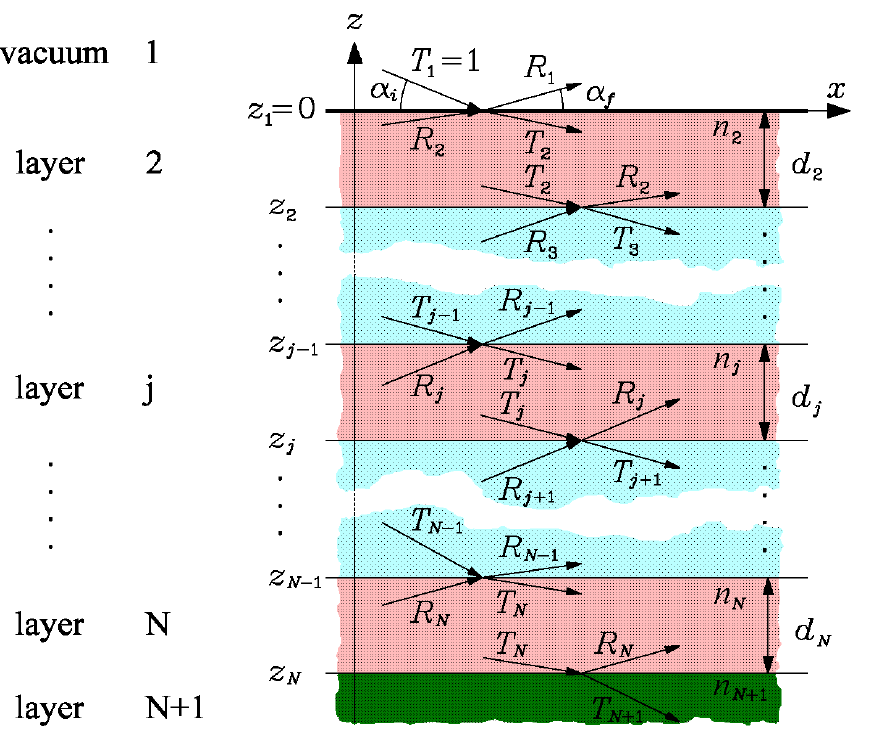
\includegraphics[width=\textwidth]{figures/parratt.png}
    \caption{Veranschaulichung der wiederholten Reflexionen bei mehreren internen Schichtübergängen, welche durch den Parratt-Algorithmus berechnet werden können.}
    \label{fig:parratt}
\end{figure}

\subsection{Messung der Rauigkeit}
Die bisherigen Überlegungen wurden alle unter der Annahme angestellt, dass die einzelnen Oberflächen alle ideal glatt sind. In der Realität besitzen Oberflächen jedoch kleine Unebenheiten, welche sie rau machen. Diese Rauigkeit sorgt für eine Abweichung vom von der Theorie postulierten Endergebnis. Um diese Abweichung zu berücksichtigen, wird eine weitere Größe eingeführt: Die \textit{Rauigkeit}
\begin{aquation}
    \sigma_j^2 &\coloneqq \int dz\left(z - z_j\right)P_j(z) \tp 
\end{aquation}
Dabei sind die $z_j$ die Ortskoordinate der $j$-ten Grenzfläche. Das Wahrscheinlichkeitsmaß $P_j$ ist ein Maß für den Anteil der Fläche, welcher in einem infinitesimalen Intervall um die Koordinate $z+z_j$ liegt. Die Rauigkeit ist also das quadratische Mittel über alle Abweichungen von der perfekten Glätte. Für eine perfekt glatte Fläche verschwindet die Rauigkeit, da hier gilt $P(z) = \delta(z)$, was genau mit der linguistischen Definition der Begriffe \textit{rau} und \textit{glatt} zusammenfällt.\\
Angewandt auf die Fresnel-Koeffizienten führt die Rauigkeit zu einem zusätzlichen Vorfaktor, sodass diese nun die Form 
\begin{aquation}
    \bar{r}_{j,j+1} &\coloneqq r_{j,j+1}\hsf e^{-2 k_{z,j}k_{z,j+1}\sigma_j^2} \\
    \bar{t}_{j,j+1} &\coloneqq t_{j,j+1}\hsf e^{\left( k_{z,j} - k_{z,j+1}\right)^2\frac{\sigma_j^2}{2}}
\end{aquation}
annehmen.\cite{RoughSurfaceReflectometry}

\section{Durchführung}
\label{sec:Durchführung}
Das hier verwendete Diffraktometer besteht aus einer Röntgenröhre auf der einen und einem Empfänger für Röntgenstrahlung auf der anderen Seite. Mittig zwischen ihnen ist ein Tisch für die Probe platziert. Zur Steuerung des Versuchsaufbau wird das Programm XRD-Commander verwendet.

\subsection{Die Röntgenröhre}
In diesem Versuch wird eine Röntgenröhre mit Cu-Anode verwendet. In dieser werden Elektronen aus einer Glühkathode in Richtung Cu-Anode beschleunigt. Die in die Cu-Anode einschlagenden Elektronen interagieren dann mit dem Kupfer, und zwar auf zweierlei Arten: Durch Stöße mit den Elektronen in den Kupferatomen werden diese auf höhere Niveaus angeregt. meistens werden die Atome sogar ionisiert. Dies macht Plätze auf niedrigeren Niveaus frei und führt damit dazu, dass Elektronen höherer Niveaus unter Emission von Röntgenstrahlung auf auf diese niedrigeren Niveaus zurückfallen. Außerdem wird bei der Bewegung der Elektronen im elektrischen Feld innerhalb des Kupfers Bremsstrahlung emittiert.\\
In diesem Versuch wird die $\text{K}_\alpha$-Linie von Kupfer verwendet, also jene Röntgenstrahlung, welche beim Niveauüübergang von der zweiten auf die erste Schale entsteht. Sie besitzt eine Wellenlänge von $\lambda=1.54\text{Å}$. Um diese aus dem restlichen Spektrum der Röntgenröhre herauszufiltern, wird ein \textit{Göbelspiegel} verwendet. Dieser bündelt die Strahlung und filtert alle anderen Linien aus der Strahlung heraus.\\
Die Strahlung fällt nach dem Göbelspiegel auf eine Blende, dann auf die Probe und dann auf eine weitere Blende. Die Blenden dienen dazu, den eingestellten Glanzwinkel der einfallenden und den gemessenen Glanzwinkel der ausfallenden Strahlung zu variieren.\\
\\
Bei sehr geringen Winkeln (kleiner als $\alpha_g$) schießt die Strahlung über die Probe hinaus. Dies äußert sich in einem reskalierenden Faktor vor der gemessenen reflektierten Intensität, dem \textit{Geometriefaktor} 
\begin{aquation}
    G &\coloneqq \left\{ \begin{matrix}
        \frac{D \sin{\alpha_i}}{d_0} & \alpha_i < \alpha_g \\
        1 & \text{sonst}
    \end{matrix} \right. \tc
\end{aquation}
mit der Probenlänge $D$ und der Strahlbreite $d_0$.

\subsection{Justage}
Da die Probe, welche hier ein mit einer dünnen Polystyrolschicht überzogener Silizium-Wafer ist, nach dem Einbringen in den Versuchsaufbau noch nicht die richtige Ausrichtung hat, muss der Aufbau zunächst justiert werden. Ziel der Justage ist es, die Probe genau mittig zwischen Sender und Empfänger zu platzieren, sodass die gesamte Strahlung der Röntgenröhre auf die Probe trifft. Außerdem muss die Nullposition für Sender und Empfänger so justiert werden, dass die Probe bei einem Glanzwinkel von null genau parallel zum Strahl steht.\\
\\
Im ersten Schritt der Justage wird daher ein Detektorscan durchgeführt. Bei diesem wird die Röntgenröhre direkt auf den Detektor gerichtet. Der Detektor wird im Winkel variiert und durch den Strahl gefahren. Das Maximum dieser Gauß-verteilten Messung wird dann als neue Null-Position eingestellt.\\
\\
Als Nächstes wird die Probe in den Strahl eingebracht. Da zuvor die der gesamte Strahl den Detektor traf, lässt sich durch Hochfahren Bewegen der Probe im Strahl der Punkt in z-Richtung bestimmen, bei welchem ungefähr der halbe Strahl abgeschattet ist. Dies wird mithilfe eines \textit{Z-Scan}s bewerkstelligt. Auf diesen Punkt wird die Probe gesetzt. Da die Feinjustage später kommt, reicht hier ein ungefährer Wert.\\
\\
Der folgende Scan dient dazu, den Einfallswinkel gleich dessen Ausfallswinkel zu setzen. Dazu werden Röntgenröhre und Detektor um die Probe rotiert, ohne ihre relative Ausrichtung zu einander zu ändern. Dieser Scan heißt \textit{Rocking-Scan} (engl. \textit{to rock}: Schaukeln). Da dieser Scan den Strahl einmal mit der dem Emitter und einmal mit der dem Detektor zugewandten Kante der Probe verdeckt, liefert er Aufschluss über die Positionierung der Probe entlang des Strahls. Das Ergebnis dieses Scans sollte ein gleichseitiges Dreieck sein. Ist dies nicht der Fall, muss die Probe entlang des Strahls verschoben werden, bis ihre Ausrichtung passt, damit später auch wirklich der gesamte Strahl die Probe trifft. Nach dieser Justage wird das Maximum des Rockingscans als neue Nulllage des Emitter-Detektor-Paars gewählt, damit der Strahl nun genau parallel zur Oberfläche der Probe steht.\\
\\
Im Anschluss wird ein weiterer Z-Scan durchgeführt, um eine präzisere halbe Abschattung des Strahls zu erreichen.\\
\\
Ein anschließender Rocking-Scan, mit einem Glanzwinkel von $0.15^\circ$ verfeinert die Parallelität der Probe zum Strahl.\\
\\
Zum Schluss wird für den selben Glanzwinkel ein letzter Z-Scan durchgeführt und die Probe wieder auf die halbe Abschattung gesetzt. Dieser sorgt dafür, dass der Strahl genau mittig auf die Probe trifft.

\subsection{Reflektivitätsmessung}
Die eigentliche Messung dient zur Bestimmung der Reflektivität. Um diese zu bestimmen, muss wie zuvor beschrieben ein Winkelbereich abgefahren werden. Dabei werden Emitter und Detektor gleichzeitig immer um den selben Glanzwinkel verschoben, um so die Intensität des reflektierten Strahls unter verschiedenen Winkel zu messen. Hier wurde ein Winkelintervall von $[0^\circ,2.5^\circ]$ gewählt, mit einer Schrittweite von $0.005^\circ$.\\
\\
Um den Untergrund der Reflektivitätsmessung zu bestimmen, wird der selbe Scan erneut durchgeführt, allerdings mit um $0.1^\circ$ verschobenem Detektor, was als \textit{diffuser Scan} bezeichnet wird. 

\section{Analysis}
\label{sec:Analysis}

The following analysis is performed with the programming language python \cite{python} and the libraries numpy \cite{numpy} for numerical calculation, scipy \cite{scipy} for curve fitting and uncertainties \cite{uncertainties} for error calculation.
Furthermore, the graphical representations are created with the matplotlib \cite{matplotlib} library.

\subsection{Dependence of the contrast on the polarisation angle}
\label{subsec:polarisation}

The first analysis step is to determine the dependence of the contrast on the polarisation angle.
For this, the maximum and minimum voltage of the photodiodes was measured in dependence of the polarisation angle.
The original measurement values are shown in figure \ref{fig:original_data} in appendix \ref{sec:appendix}.
The mean values of the measurements and the with equation (\textbf{HIER FORMEL EINFÜGEN}) calculated contrast is shown in table \ref{tab:values_polarisation}.

\begin{table}[H]
    \centering
    \caption{Measured Values of the contrast in dependence on the polarisation angle.}
    \label{tab:values_polarisation}
    \begin{tabular}{c c c c}
        \toprule
        $\vartheta \,/\, \si{\degree}$ & $I_{\text{max}}\,/\,\si{\volt}$ & $I_{\text{min}}\,/\,\si{\volt}$ & contrast \\
        \midrule
        0.0 & $4.98$ & $4.52\pm0.01$ & $0.05$ \\
        15.0 & $4.37\pm0.02$ & $2.35\pm0.01$ & $0.30$ \\
        30.0 & $3.91$ & $1.15\pm0.01$ & $0.55$ \\
        45.0 & $4.45$ & $0.81$ & $0.69$ \\
        60.0 & $5.86\pm0.01$ & $1.07\pm0.01$ & $0.69$ \\
        75.0 & $6.53\pm0.05$ & $2.29\pm0.01$ & $0.48$ \\
        90.0 & $7.10\pm0.05$ & $5.38\pm0.04$ & $0.14$ \\
        105.0 & $9.92\pm0.11$ & $4.42\pm0.07$ & $0.38\pm0.01$ \\
        120.0 & $13.15\pm0.13$ & $2.71\pm0.04$ & $0.66$ \\
        135.0 & $17.61\pm1.42$ & $1.65$ & $0.83\pm0.01$ \\
        150.0 & $12.94\pm0.10$ & $2.53\pm0.01$ & $0.67$ \\
        165.0 & $9.87\pm0.08$ & $3.86\pm0.03$ & $0.44$ \\
        180.0 & $5.33\pm0.04$ & $4.78\pm0.01$ & $0.05$ \\
        \bottomrule
    \end{tabular}
\end{table}

\noindent
A graphical representation of the contrast in dependence on the polarisation angle is shown in figure \ref{fig:contrast}, while a theroetical prediction of the form
\begin{align}
    K = 2K_0\cdot|\sin(\vartheta-\delta)\cdot\cos(\vartheta-\delta)|
\end{align}
is fitted to the data.
The offset of $\delta$ that is used to compensate for deviations of the experimental setup and the amplitude $K_0$ are determined to be
\begin{align*}
    K_0=\SI{0.697\pm0.004}{} \quad \text{and} \quad \delta=\SI{1.620\pm0.010}{\degree}.
\end{align*}
For the following measurements, the polarisation angle is set to $\SI{135}{\degree}$, as this angle provides the highest contrast.
\begin{figure}[H]
    \centering
    \includegraphics[width=0.75\textwidth]{build/contrast.pdf}
    \caption{Graphical representation of the contrast in dependence on the polarisation angle.}
    \label{fig:contrast}
\end{figure}

\subsection{Refraction index of glass}
\label{subsec:refraction_glass}

In order to analyse the refractive index of the glass, a total of five series of measurements were carried out in which the angle of the glass plate was varied by $\SI{10}{\degree}$.
The measurements of the refraction index of glass are shown in table \ref{tab:refraction_glass}, giving a mean value of $\#M=\num{33.4\pm1.4}$.
\begin{table}[htbp]
    \centering
    \begin{tabular}{c c c}
        \toprule
        Measurement series & $n$ \\
        \midrule
        1 & 31 \\
        2 & 34 \\
        3 & 34 \\
        4 & 33 \\
        5 & 35 \\
        \bottomrule
    \end{tabular}
    \caption{Measured counts for the refraction index of glass for different measurement series with $\upDelta \vartheta=\SI{10}{\degree}$.}
    \label{tab:refraction_glass}
\end{table}
To calculate the refraction index of glass, equation (\textbf{HIER FORMEL EINFÜGEN}) is simplified to the form
\begin{align}
    % \bar M = \frac{d}{4\pi^2\lambda}\cdot \left(\frac{n-1}{2n}\cdot \Theta^2 \cdot \underbrace{\theta}_{\text{tilted glass plate}}\right),
    n = 1+ \frac{\#M\cdot\lambda}{d}
\end{align}
where $d$ denotes the thickness of the glass plate, $\lambda$ the wavelength of the light in vacuum and $\#M$ the measured maxima.
The refraction index of glass is then calculated to be $n=\num{1.37\pm0.06}$. %$M=\num{4.074\pm0.005}$.

\subsection{Refraction index of air}
\label{subsec:refraction_air}

The refraction index of air is determined by measuring the number of maxima in dependence of the pressure.
The original measurement values are shown in figure \ref{fig:original_data} in appendix \ref{sec:appendix}, while the mean values of the 3 measurement series are shown in table \ref{tab:refraction_air}.
\begin{table}[htbp]
    \centering
    \begin{tabular}{c c}
        \toprule
        pressure / $\si{\milli\bar}$  & counts \\    
        \midrule
        50.0 & $2.0$\\
        100.0 & $4.0$\\
        150.0 & $6.0$\\
        200.0 & $8.0$\\
        250.0 & $10.0$\\
        300.0 & $12.0$\\
        350.0 & $14.0$\\
        400.0 & $16.0$\\
        450.0 & $18.5\pm0.6$\\
        500.0 & $21.0$\\
        550.0 & $23.0$\\
        600.0 & $25.0$\\
        650.0 & $27.0$\\
        700.0 & $29.0$\\
        750.0 & $31.0\pm0.6$\\
        800.0 & $33.0\pm0.6$\\
        850.0 & $36.0$\\
        900.0 & $38.0$\\
        950.0 & $40.0$\\
        1000.0 & $42.0$\\
    \end{tabular}
    \caption{Measured counts for the refraction index of air in dependence of the pressure.}
    \label{tab:refraction_air}
\end{table}


\begin{figure}[H]
    \centering
    \includegraphics[width=0.75\textwidth]{build/refraction_index.pdf}
    \caption{Graphical representation of the refraction index of air in dependence of the pressure.}
    \label{fig:refraction_index}
  \end{figure}
\section{Diskussion}
\label{sec:Diskussion}
\subsection{Der invertierende Verstärker}
Die gemessenen Leerlaufverstärkungen liegen alle außerhalb der Standardabweichung. Da die Abweichung jedoch bei allen drei Widerständen um eine ähnliche Abweichung niedriger als der Theoriewert ist, liegt der Schluss nahe, dass der Gesamtwiderstand im Bereich des Widerstandes $R_1$ (vgl. \autoref{fig:inverting-OpAmp}) nicht vernachlässigbar ist.\\
Denn zum Einen würde ein erhöhter Widerstand im Bereich von $R_2$ die Abweichung nach unten weiter erhöhen, statt sie zu verringern, wie leicht aus der so modifizierten Verstärkung 
\begin{aquation}
    V &= \frac{R_2}{R_1} \rightarrow \frac{R_2 + R_\text{sys}}{R_1}
\end{aquation}
zu erkennen ist.\\
Eine Abweichung im Bereich von $R_1$, sodass 
\begin{aquation}
    V &= \frac{R_2}{R_1} \rightarrow \frac{R_2}{R_1 + R_\text{sys}}
\end{aquation}
hingegen würde auch erklären, warum die relative Abweichung mit abnehmendem $R_2$ kleiner wird, denn je kleiner $R_2$, desto schwächer wird in diesem Fall die Gewichtung bei der Berechnung der relativen Abweichung.\\
Eine Überschlagsrechnung mit geschätzten Werten ergibt, dass eine Modifikation des Theoriewerts von $R_1$ um $R_\text{sys} = 0.25 \kOhm$  den größten Teil der Abweichung tatsächlich sehr gut erklären kann.\\
\begin{table}[h!]
    \centering
    \begin{tabular}{|>{$}c<{$}|>{$}c<{$}|>{$}c<{$}|}
    \hline
    V_{\text{Theorie}} & V_{\text{Leerlauf}} & \text{relative Abweichung} \\ \hline
    220 & 174.64 \pm 2.61 & 20.6\% \\
    150 & 123.26 \pm 1.29 & 17.8\% \\
    100 & 84.70 \pm 1.04 & 15.3\% \\
    \hline
    \end{tabular}
    \caption{Vergleich der Ergebnisse des invertierenden Verstärkers}
    \label{tab:ergebnisse_verstärkung_vergleich}
\end{table}
Da die Grenzfrequenz von der Verstärkung abhängt und die Bandbreite von der Grenzfrequenz, pflanzt sich dieser Fehler in diese fort, sodass sie ebenfalls angepasst werden müssen.

\subsection{Integrator und Differentiator}
Die Messungen der Zeitkonstante des Integrators und des Differentiators sind beide weit abseits der theoretischen Prognosen. Ein sehr naheliegender Grund dafür könnten falsch eingebaute Bauteile sein. Unter den vorhandenen Bauteilen befanden sich nämlich Widerstände mit $10\kOhm$ und $100\kOhm$ und Kondensatoren mit $22 \text{nF}$ und $100 \text{nF}$.\\
Beim Integrator würde der versehentliche Einbau eines Widerstandes mit $100\kOhm$ statt, wie geplant eines Widerstandes mit $10\kOhm$ die Abweichung in Kombination mit dem aus der Abweichung des invertierenden Verstärkers geschlossenen abweichenden Widerstand des Gesamtaufbaus relativ gut erklären, denn damit würde
\begin{aquation}
    {RC}_\text{$\int$,theo} &= 1 \text{ms} &\rightarrow 10 \text{ms} &\tc\\
    {RC}_\text{exp} &= (8.90 \pm 0.27) \text{ms} \tp
\end{aquation}
Für den Differentiator würde ein falsches Bauteil, nämlich der Vertausch eines Kondensators mit $C = 22 \text{nF} \rightarrow 100 \text{nF}$
\begin{aquation}
    {RC}_\text{$\partial$,theo} &= 22 \text{ms} &\rightarrow 100 \text{ms}&\tc \\
    {RC}_\text{exp} &= (79.85 \pm 10.98) \text{ms}
\end{aquation}
ebenfalls gut erklären.

\subsection{Der Schmitt-Trigger}
Beim Schmitt-Trigger sind die experimentellen Ergebnisse sehr nah an den theoretisch prognostizierten.

\subsection{Der (variable) Generator}
Die aus den Daten zum variablen Generator bestimmte Periodendauer $T = (5.58 \pm 0.19) \text{ms}$ weicht um $11.1\%$ vom Theoriewert $T_\text{theo} = 6.28 \text{ms}$ ab. Da die Periodendauer direkt proportional zur Zeitkonstante $RC$ und damit zum Widerstand $R$ ist, ist dies ein weiterer Hinweis darauf, dass der Widerstand der Leitung vor den Generatorkomponenten größer ist als gedacht, denn dies würde direkt die Zeitkonstante und damit die Periodendauer vergrößern.




\printbibliography{}

\appendix
\newpage

\section{Appendix}
\label{sec:appendix}

Original data sheets wirth the entire data can be found in picture \ref{fig:original_data}.
The measurements that are shown in table \ref{tab:values_polarisation} and table \ref{tab:refraction_air} show the respective mean values of the measurements.

\begin{figure}[H]
    \centering
    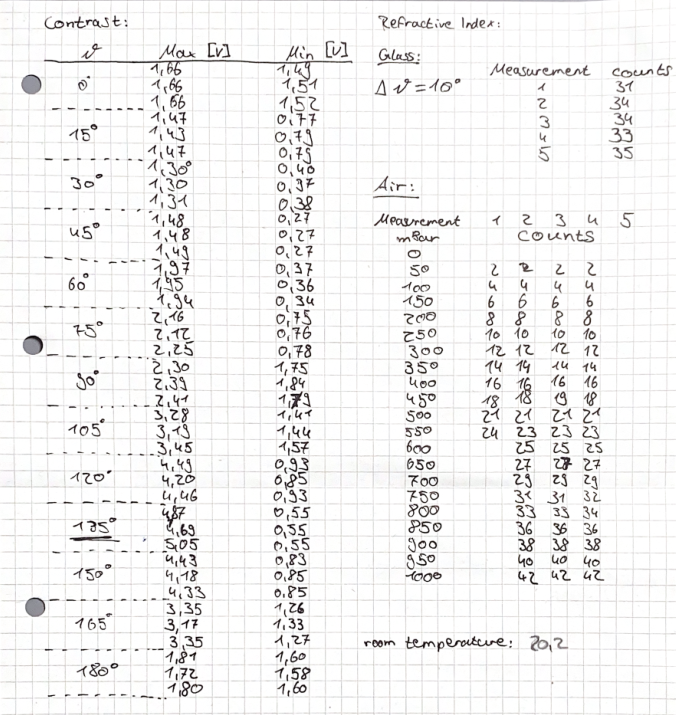
\includegraphics[width=0.75\textwidth]{./data/Messwerte.pdf}
    \caption{Original data sheets with the entire data.}
    \label{fig:original_data}
\end{figure}


\end{document}
